\chapter{Background}

In this chapter we will discuss concepts and technologies used to develop our system.

\section{Non-Volatile Memory and Persistent Memory}
    
    \subsection{Definitions}
        \NVM (NVM) is a class of memory storage devices which are able to keep data after power outage.
        There are two main categories of NVM: electrically addressed and mechanically addressed.\\
        \PM (PM) is a directly byte-addressable, non-volatile memory which can be accessed by the memory bus. %kn "via" the memory bus?
    
    \subsection{Access to NVM \cite{PmemAccess}}
        In most computer applications access to data storage proceeds as follows:
        \begin{itemize}
            \item Application uses the file system API to access the files
            \item File system performs read and write operations through a driver
            \item All data transferred during those operations is composed of blocks, typically of size 4KB
        \end{itemize}
        Solution described above is inadequate from the point of view of PM, because it makes programmers unable to use its byte-addressability. % from the PM point of view - nie lepiej?
        To solve this problem method called \DAX (DAX) was created.
        In this approach persistent memory-aware file system is used to map virtual addresses to physical addresses in PM. 
        It allows applications to access directly to individual bytes of the storage.
      
    \subsection{Emulation \cite{PmemEmulation}}
        Emulation of the \PM is not obligatory during the development of the project, however, it is required to achieve a sufficient performance of the final product. 
        Emulation is based on DRAM memory, which is recognized by operating system as persistent memory region.
        \PM emulated in such way will not keep data after power outage, but it will provide performance comparable with hardware solution.
        
    \subsection{Programming for NVM}
        Programming for persistent memory differs from programming for volatile memory. 
        In case of this project there are two most important differences that should be considered.
        
        Firstly, persistent memory is not reinitialized after the application restart. 
        It implies that corrupted or incomplete data is kept in data structure and may cause incorrect functioning of the program or crashes. 
        To prevent such situations transactions or similar mechanism must be provided.
        
        Second problem is a synchronisation mechanism. 
        Using mutexes in persistent memory may cause unintended behaviour. 
        If a thread crashes after locking a mutex, it may never unlock which results in a deadlock. 
      
\section{Persistent Memory Development Kit}

    \subsection{Overview}
        Persistent Memory Development Kit (PMDK) \cite{PmemIo} is a set of libraries developed by Intel Corporation, which aim is to support persistent memory programming. 
        It is based on memory-mapped files (POSIX mmap() system call). 
        PMDK consists of 10 libraries suitable for various tasks, most important of which are described below. 
        It also includes examples which demonstrate how to use each of those libraries and their documentation.
        
    \subsection{Libpmem library}
        Libpmem library provides a low-level persistent memory API for C language. 
        It requires developers to handle memory allocation and flushing changes to persistent memory by themselves. 
        It also does not provide transactions.
        Other libraries included in PMDK are based on libpmem and call it internally.
    
    \subsection{Libpmemobj library}
        Libpmemobj is a high-level persistent memory library providing API for C language.
        In contrast to libpmem library, it has implementations of some high-level concepts: 
        \begin{itemize}
            \item Persistent memory management - persistent memory allocation mechanism and persistent memory pointers are provided.
            \item Transactions - memory snapshot is created and can be restored after failure of a transaction block.
            \item Concurrency support - API similar to pthread API allows to use mutexes which are automatically unlocked when a crash occurs.
            \item Data structures - non-transactional doubly-linked list similar to the one implemented in C standard library is provided. 
        \end{itemize}
        
    \subsection{Libpmemobj++ library}
        Libpmemobj++ library provides a C++ bindings for libpmemobj.
        It allows to create object-oriented applications providing API similar to C++ Standard Template Library (STL), including smart pointers and mutexes compatible with STL locks (std::shared\_lock, std::unique\_lock). % dodaj zrodla, chyba juz nawet sa w biblio dla rozdzialu 3go
        Unfortunately it does not support polymorphism, so objects stored in persistent memory cannot use this mechanism.
    
\section{Distributed hash table} % distributed hash table

    This section covers the general concepts of creating a distributed system for the implemented data structure.

    \subsection{Assumptions}
        The project assumption is to create a distributed system consisting of many nodes working on the same hash map.
        Each one can operate on the hash map through its read and write operations.
        The nodes can join or leave the system at any time without any negative consequences for the data integrity.
        The data shall have high availability, which is one of the most important components of the CAP theorem \cite{CAP}.
        That means that the client has to get a response regardless of the state of any node in the system.
        Achieving high availability requires the system to have no downtimes and to be operational all the time.
        Given the above assumptions, we decided to follow the rules introduced by Amazon in their solution: \Dynamo \cite{AmazonDynamo}.
    
    \subsection{Amazon Dynamo}
        Since Amazon is one of the largest e-commerce companies, their services are used by millions of users concurrently. 
        Their platform consists of tens of thousands of servers and network components located around the world. 
        In such architecture single units failures are inevitable and have to be taken into account when creating the system.
        % For such an enterprise even a small system failure could lead to enormous financial consequences and losing customer trust. 
        
        \Dynamo is highly available key-value storage system.
        It is used by some core services of Amazon to provide the "always-on" experience, for example Amazon Simple Storage Service \cite{AmazonS3} also known as Amazon S3.
        In Dynamo the key principles are:
        
        \begin{itemize}
            \item \textit{Incremental scalability}:
                The system should be able to scale out easily.
                Connecting a new node to the network cannot have a significant impact on the system performance.
            \item \textit{Symmetry}:
                Each node in the system is equal and has the same set of responsibilities as its peers. 
                There is no superior unit to control the system, so that its maintenance is simplified.
            \item \textit{Decentralisation}:
                This is an extension of the symmetry principle.
                A centralised control of the system could result in an outage and be a bottleneck of the whole network.
                Therefore, decentralised peer-to-peer techniques should be favoured during development.
                It can lead to better scalable system with higher availability.
            \item \textit{Heterogeneity}:
                The system should be implemented in a way that allows control of work distribution. 
                The amount of work given to a node should be proportional to its computing capabilities.
        \end{itemize}

    \subsection{Consistent hashing}
        As previously stated, the described system is composed of many nodes. 
        Their number varies constantly, since the nodes may join and leave the at any time.
        This requires different approach when distributing the hashtable between the nodes.
        Traditional method causes nearly all keys to be remapped when a new node appears.
        This would have a catastrophic impact on our system performance since the various elements in the hash table would have to constantly migrate from one node to another.
        
        A provided solution is called \textit{consistent hashing}.
        It is a concept based on creating a hash ring and mapping each object to a specified place on the ring. 
        The place is defined by a hashed key of the element.
        The minimal hash ring index corresponds to the \ang{0} angle and the maximum possible index to the \ang{360} angle.
        To assign the hashmap parts to nodes, we have to place both hashmap elements and nodes on the same ring.
        To find out what keys is a node responsible for, we need to locate the node on the circle by its hash value and move in the ascending angle direction until we find another node. 
        All objects encountered on this road belongs to this node.
        Each hashmap object belongs to the node which key is the closest to the object's key in a specified direction (clockwise or counterclockwise). 
        
        To be more consistent and distribute keys evenly among nodes, we can assign nodes not to one but to many places.
        The number of one node keys, known as \textit{weight}, depends on the situation and may be different for each node depending of its capabilities (\textit{heterogeneity}). 
        Thanks to this solution we can easily add or remove nodes to the system and only $\frac{K}{n}$ keys need to be remapped, where $K$ stands for the number of keys and $n$ for the number of nodes.
        
        \begin{figure}[ht]
            \centering
                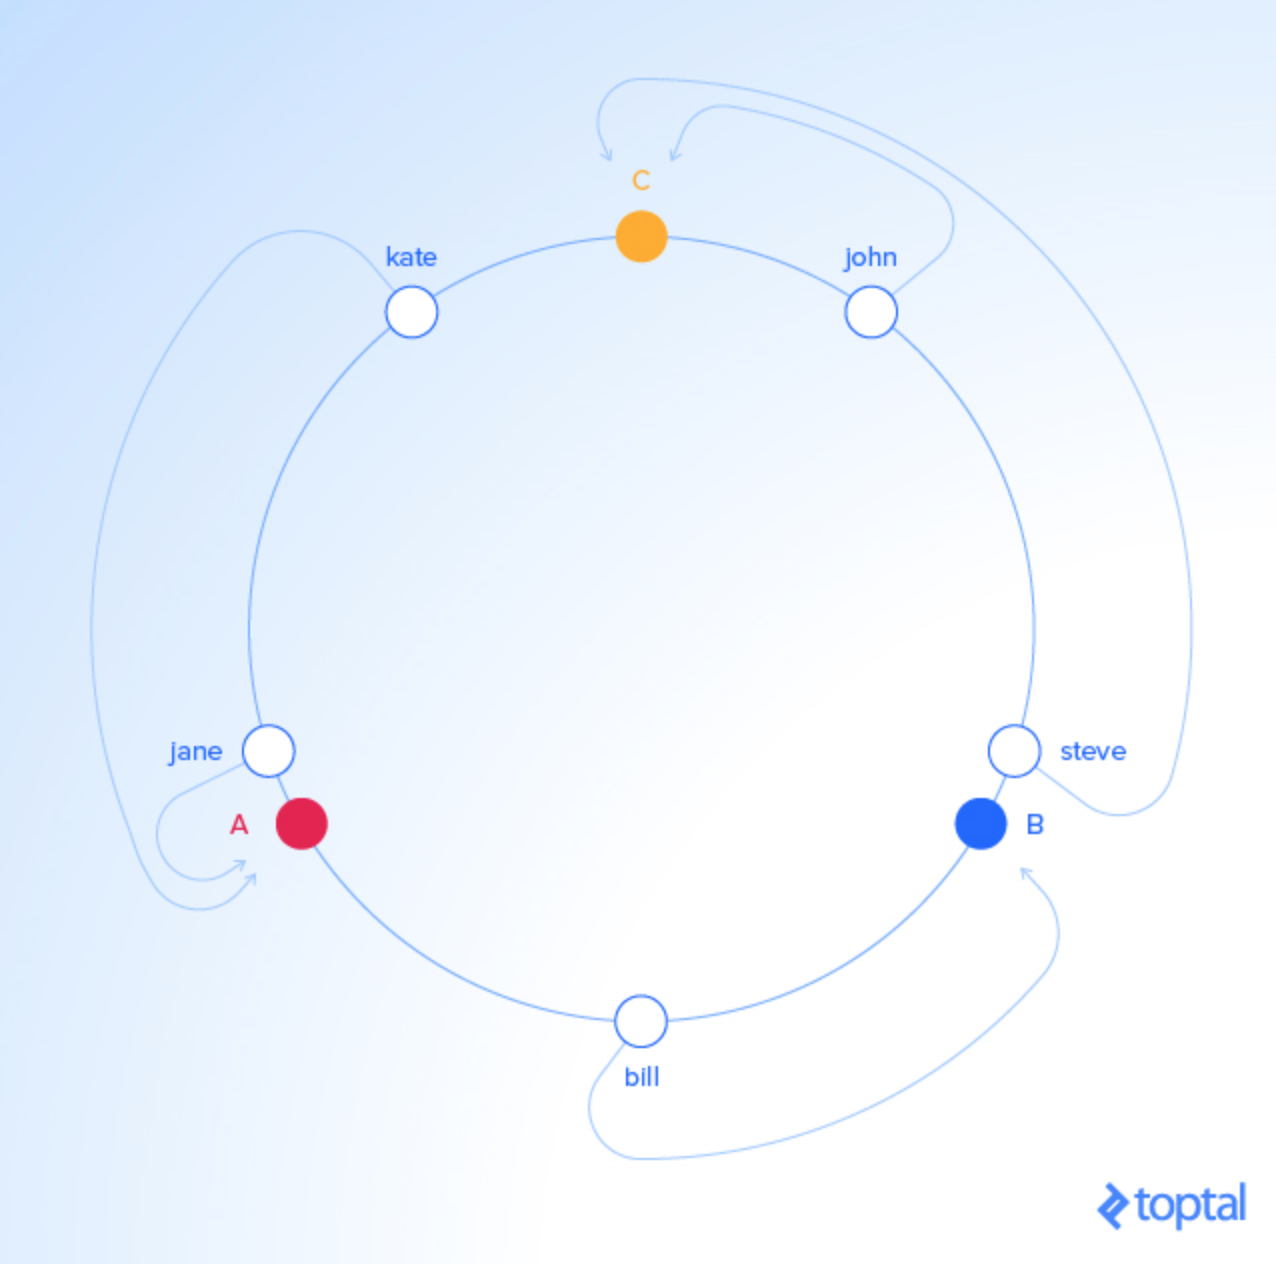
\includegraphics[width=0.45\textwidth]{thesis/figures/hashring.png}  
                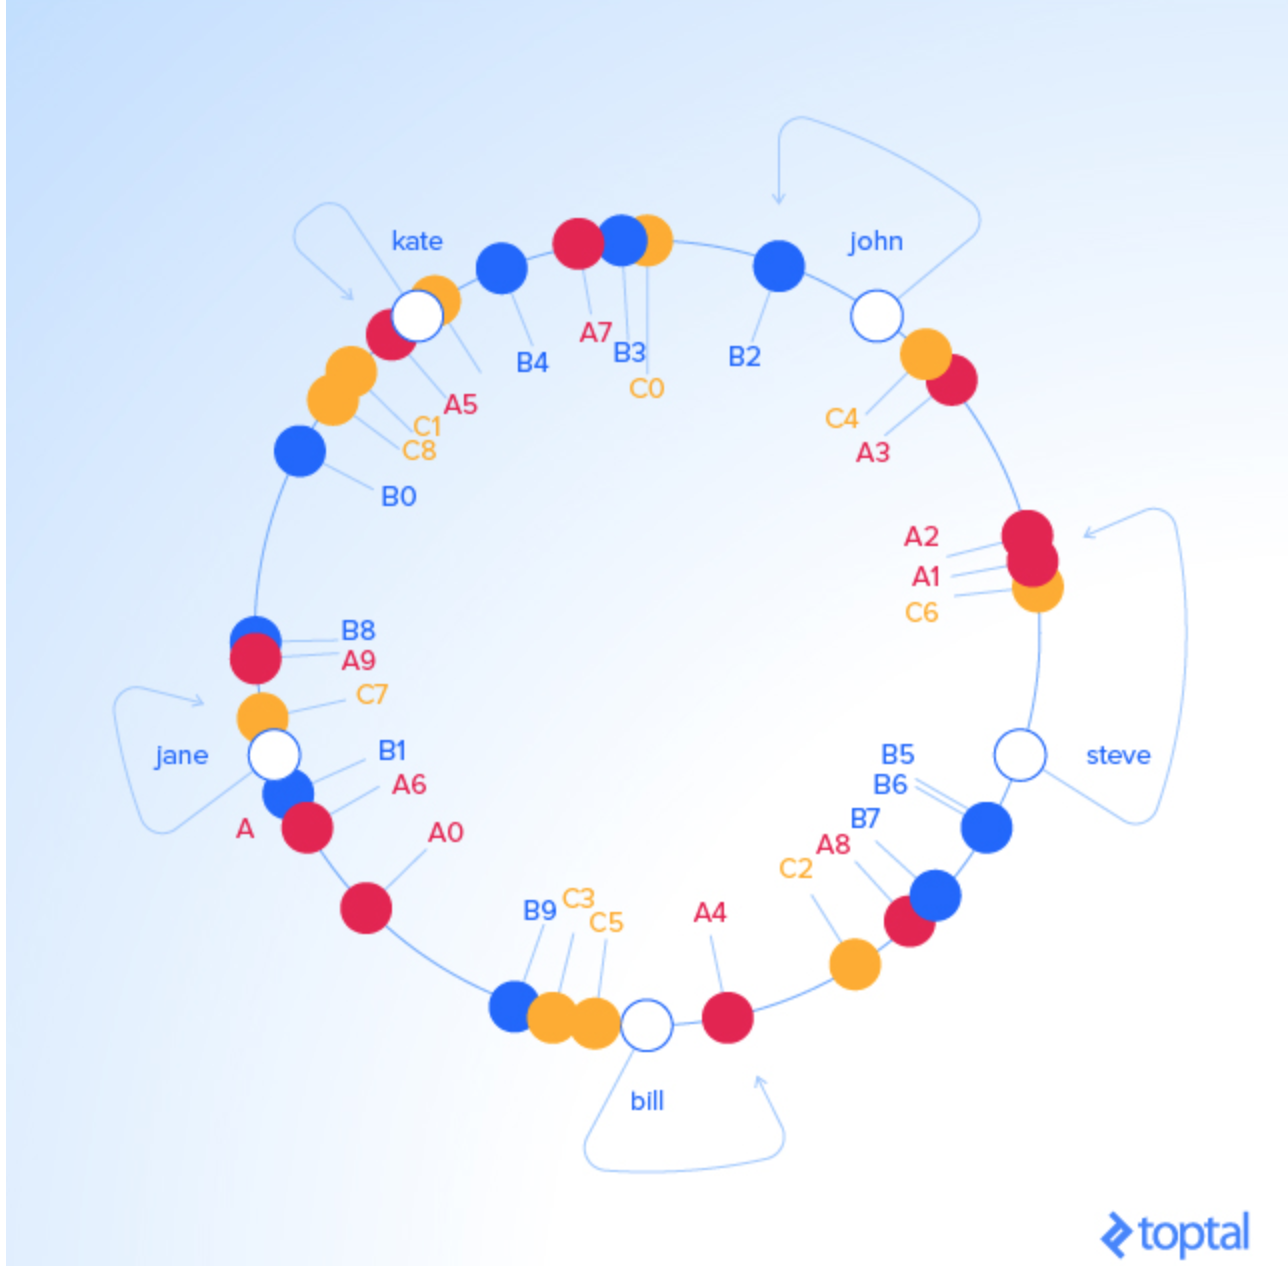
\includegraphics[width=0.45\textwidth]{thesis/figures/vnodes.png}
            \caption{Hash ring - names represents objects and letters represent nodes. 
                    Left - nodes represented once at hashring.
                    Right - nodes with many labels. \cite{ConsistentHashing}}
        \end{figure} %kn: if you want to include these pictures, i think you should describe them
        
    \subsection{Replication} 
        Since distributed systems can fail at any time we need to provide an error prone solution.
        When one of the nodes goes down the whole data it kept is lost.
        This situation is unacceptable in a distributed system.
        Solution to that is keeping replicated data across the nodes.
        For that idea we declare \textit{replication factor} which determines how many times we replicate data.
        With existing \textit{hash ring} every node knows about his neighbours.
        Every node has a copy of his local data in the number of neighbouring nodes depending on that factor.
        Thanks to that when one node becomes unavailable, we can still ask another node about data it kept.
        
    \subsection{Used libraries}
        For development purpose we wanted to use the best available solution.
        We have looked through different libraries and frameworks and decided to give a try two of them.
        \subsubsection{Seastar}
            \Seastar\cite{Seastar} is an event-driven framework allowing user to write non-blocking, asynchronous code.
            It has support for highly efficient complex server applications on modern multi-core machines.
            Most known use case of \Seastar is ScyllaDB\cite{ScyllaDB} which achieves higher throughputs and lower latencies than her role model Appache Cassandra\cite{Cassandra}.
            \Seastar use two concepts of asynchronous programming which are \textit{futures} and \textit{continuations}.
            Multicore machines have usually a huge overhead for sharing data because of that \Seastar use the share-nothing programming model.
            
            
        \subsubsection{Boost Asio}
            Asio\cite{Asio} is a C++ library for network programming with a consistent asynchronous model which offers:
            \begin{itemize}
                \item Portability - supports commonly used operating systems.
                \item Scalability - scale to thousands of concurrent connections.
                \item Efficiency - minimise data copying.
                \item BSD sockets
            \end{itemize}

            \textbf{Difficulties}:
                For the first glance \Seastar was the perfect choice for our application.
                Unfortunately we have met many problems with it.
                First of all whole building and configuring process is incomplete.
                The biggest problem was that \Seastar is not well known framework and we couldn't find any help on the internet.
                Nonetheless, after trying different operating systems and Docker we finally managed to get running \Seastar program.
                Next fact was that tests provided by \Seastar were failing on our machines.
                We wanted fully operating framework so we had to solve it again.
                Solution for that was Opera 27 which caused no problems in configuring and running tests.
                With fully operational \Seastar we started development.
                Another problem was that documentation of \Seastar covers about 10\% of all functions that they provide.
                There were some sample codes provided by \Seastar so we used reverse engineering to understand and explore source code.
                During merging NVM Hash Table application with \Seastar framework we have reached final conflict.
                \Seastar framework during it's initialization changes the \textit{hugepages}\cite{Hugepages} size which causes \textbf{Segmentation fault} on creating Persisten Memory Object.
                This difficulty was not resolved and we resigned using \Seastar any more.


%TODO Replication factor, seastar lib